\chapter{Technische Umsetzung}

Der Protoyp wurde in den Programmiersprachen Java und C++ entwickelt. Java wurde für die Orchestrierungsschicht und
Nutzeroberfläche genutzt, während C++ für die Firmware auf dem ESP32 genutzt wurde. Als EPK-Schicht wurde eine modifizierte 
Version der ARIS Produktgruppe genutzt. 

\section{Eigenentwickelte Automationsschnitstelle}

Die Automationsschnitstelle besteht aus dem EPK-Compiler, der Exeuction-Engine so wie der IoT-Schnittstelle.
Als Eingabe bekommt die Schnittstelle das EPK-Prozessmodell als XML-Datei, welche dann vom EPK-Compiler kompiliert und von 
der Exeuction-Engine ausgeführt wird, welche die Befehle an die Mikrocontroller über die IoT-Schnittstelle verschickt.

Zur Realisierung der Automationsschnitstelle wurden die folgenden Klassen implementiert:

\textbf{Prozessmodell}

\begin{figure}[H]
    \centering
    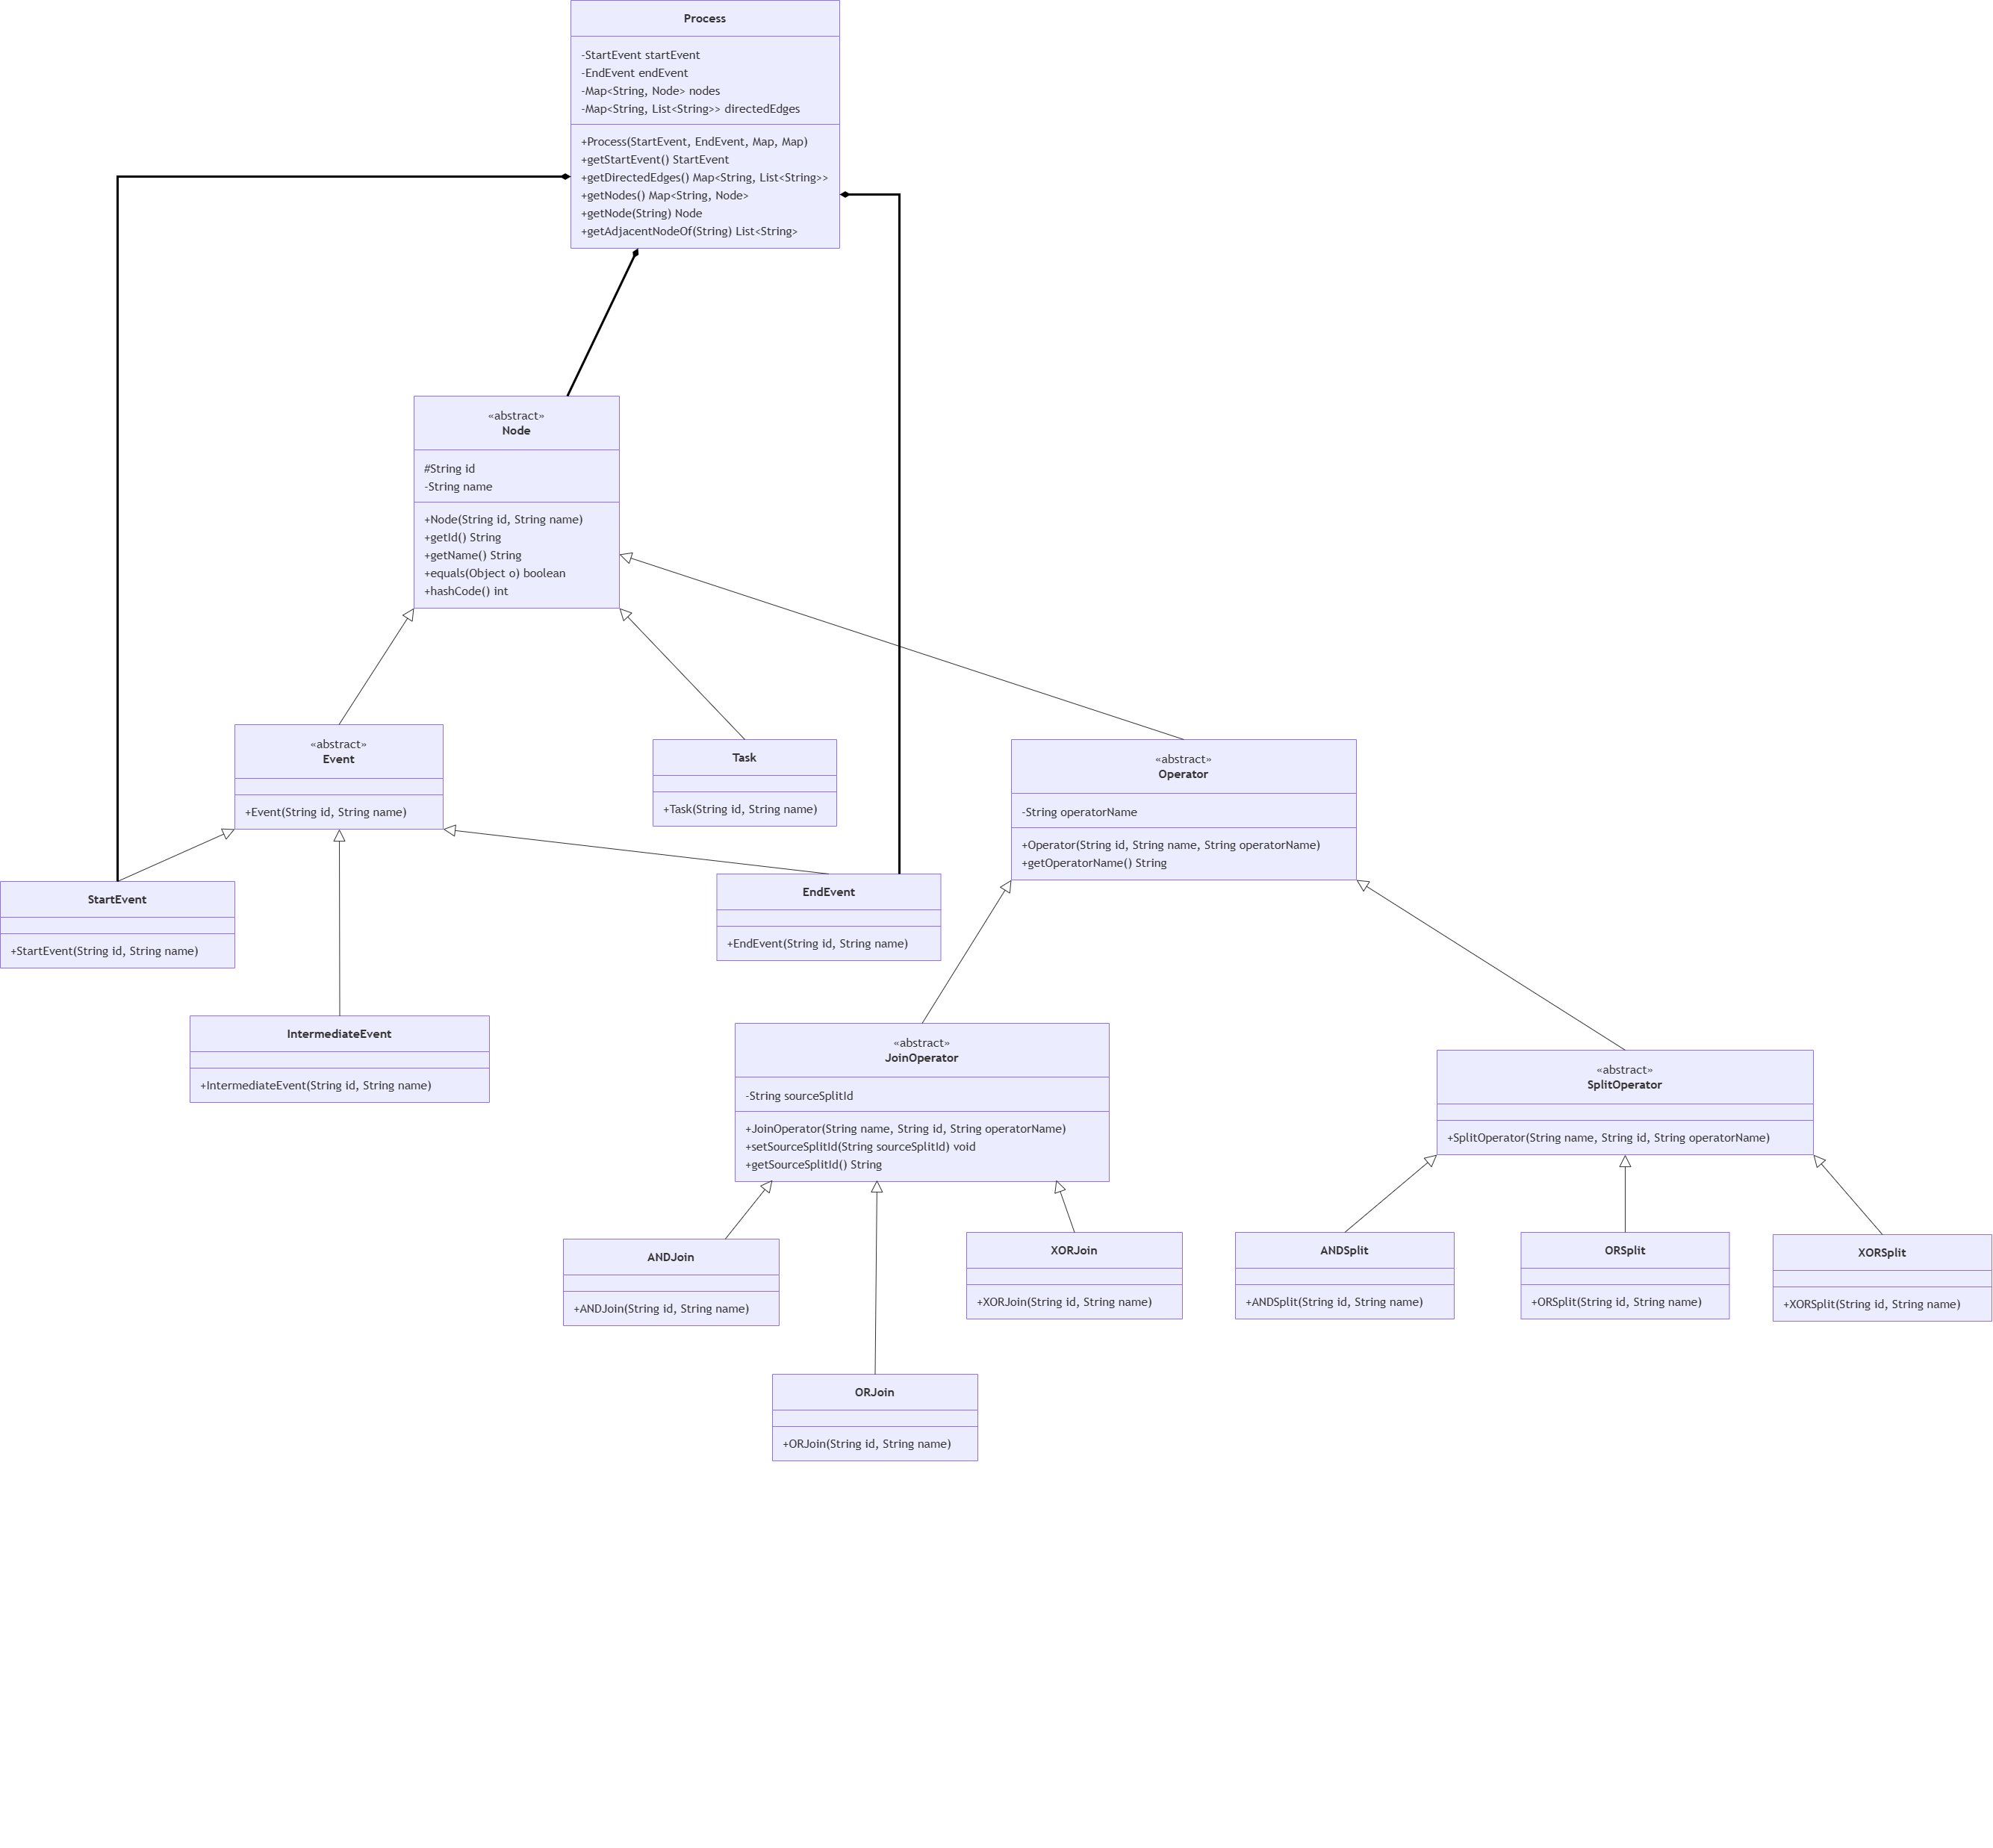
\includegraphics[width=0.8\textwidth]{Graphics/Prozess-UML.png}
    \caption{UML Diagramm der Prozessmodellimplementierung}
    \label{fig:prozess-uml}
\end{figure}

Die Klasse \texttt{Process} beschreibt das Prozessmodell $P$ und der Graph $G_P$ wird durch eine Adjazenzliste realisiert. 
Zu Kompilierungszwecken werden das Start- und Endereignis in der Klasse als Attribute hinterlegt. Die Knotenmenge $V$ wird durch die Klasse 
\texttt{Node} realisiert. Dabei wird die Teilmengenbeziehung von $E$, $O$ und $F$ durch Vererbung in Java umgesetzt. 

\textbf{Ausführungsmodell}

\begin{figure}[H]
    \centering
    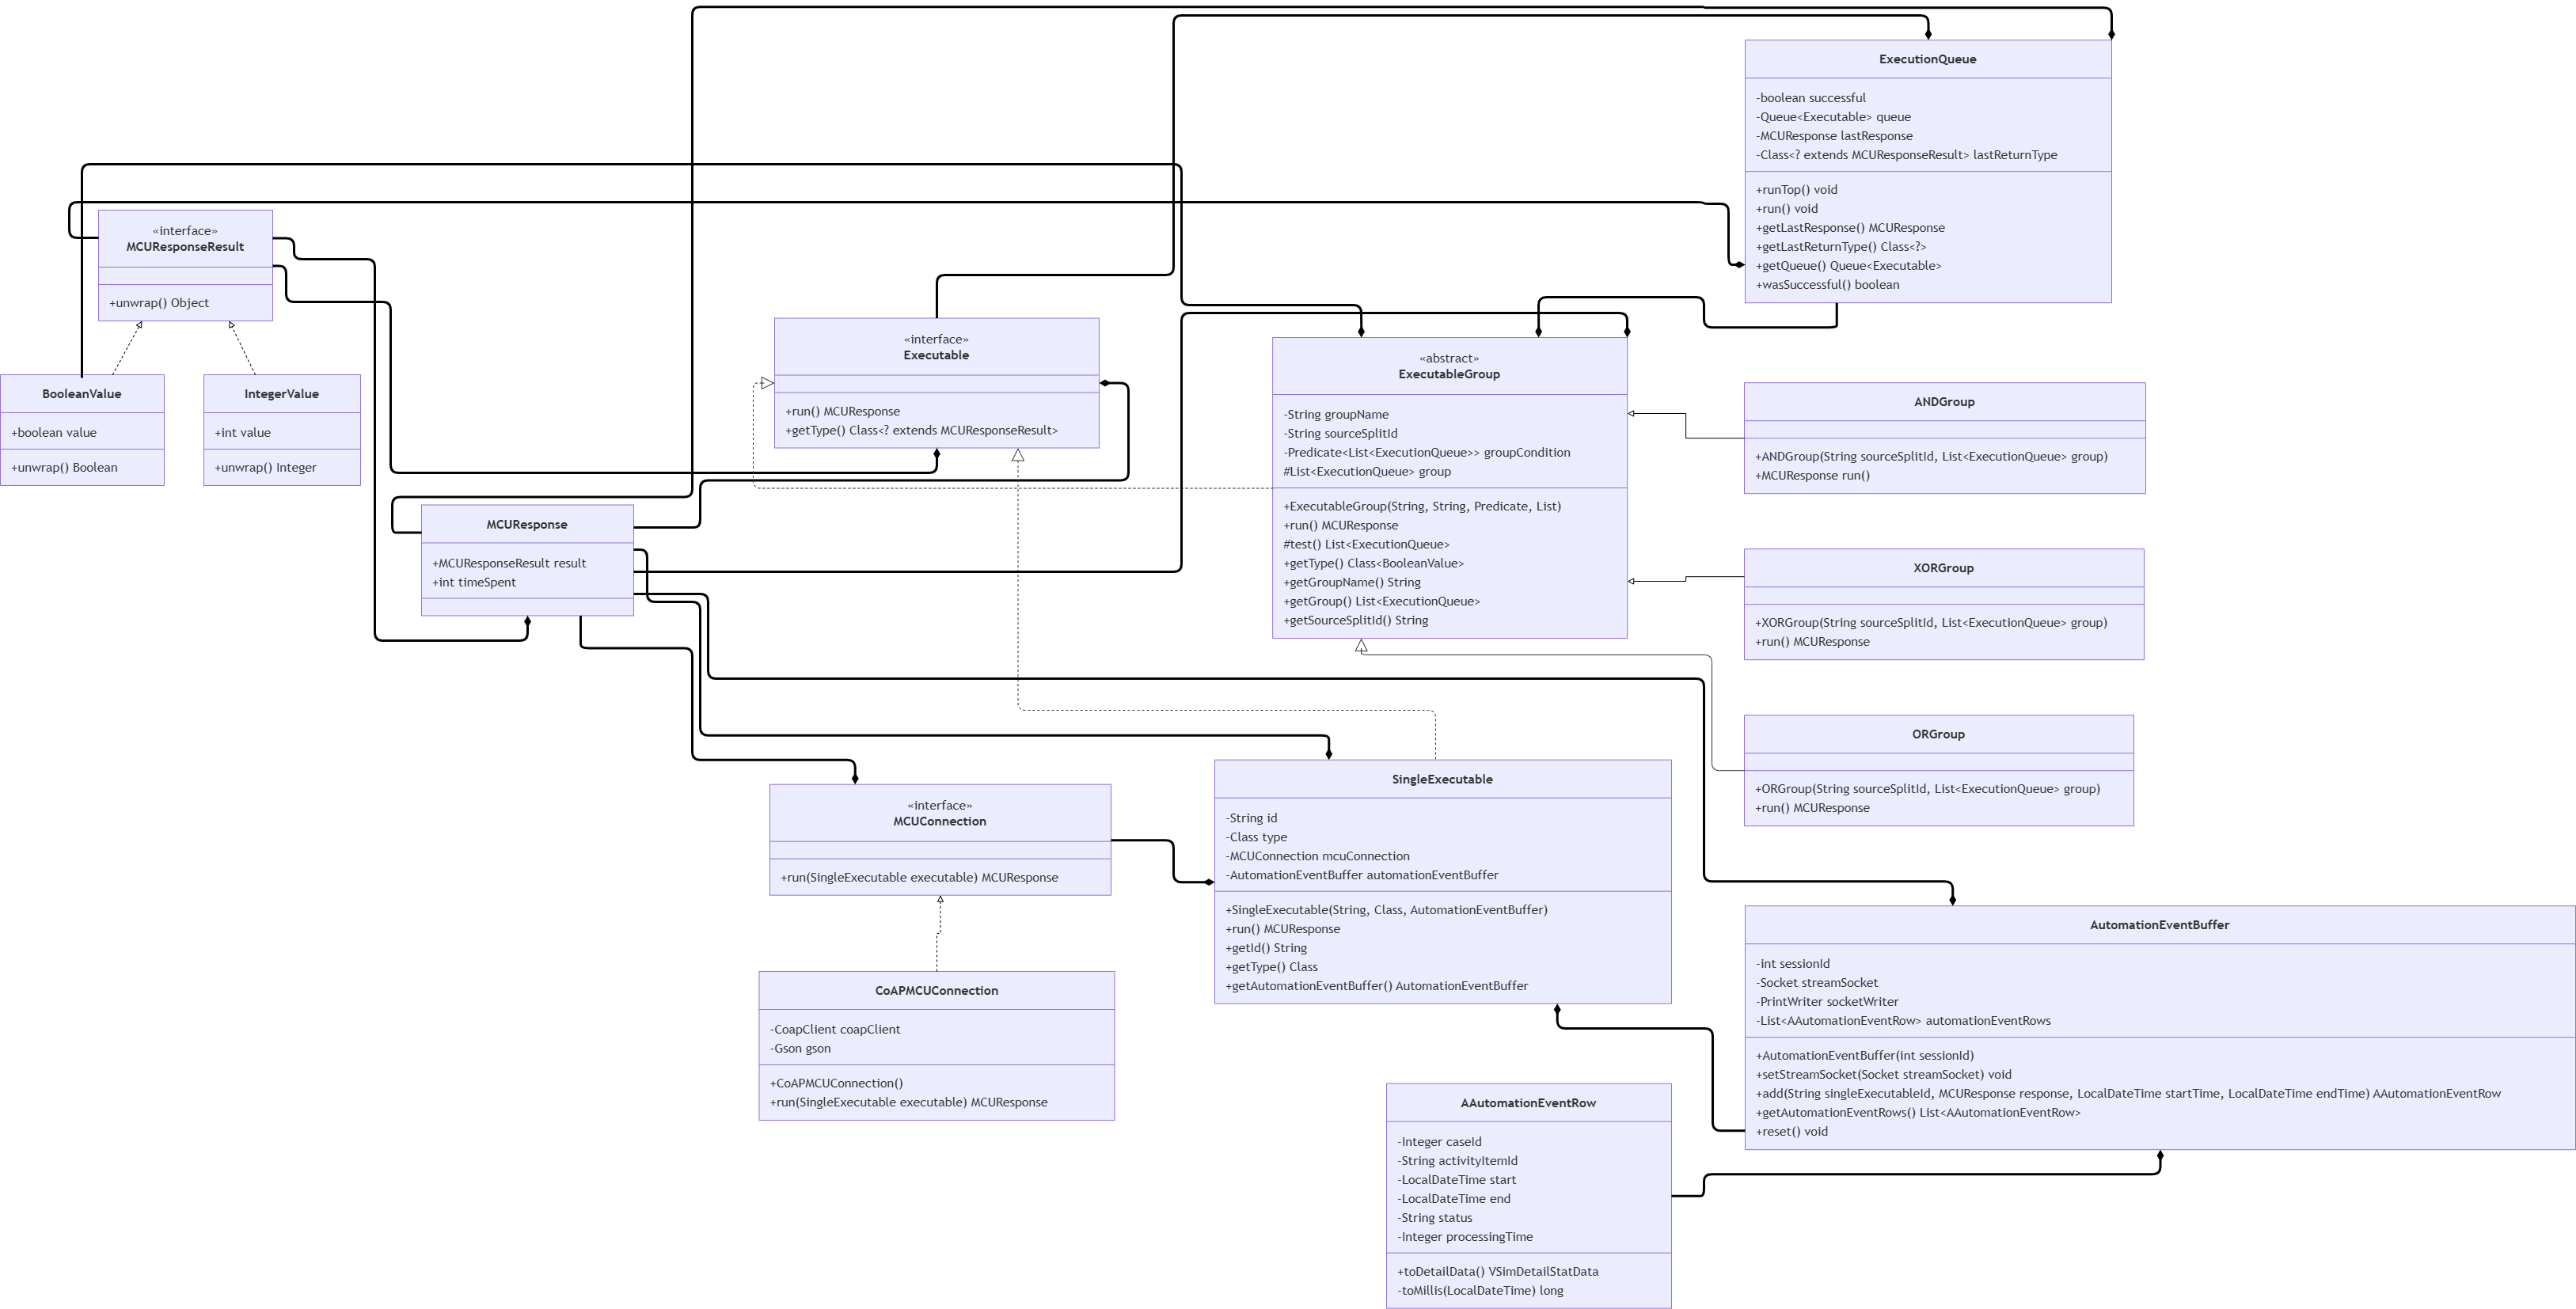
\includegraphics[width=0.8\textwidth]{Graphics/Ausführungsmodell-UML.png}
    \caption{UML Diagramm des Ausführungsmodellimplementierung}
    \label{fig:executable-uml}
\end{figure}

Die Klasse \texttt{ExeuctionQueue} implementiert das Ausführungsmodell, welche eine ExecutionQueue aus $X^*$ darstellt. Analog zu dem Modell gibt es 
die Klassen \texttt{SingleExecutable} und \texttt{ExeuctionGroup}. Zur Kommunikation mit dem IoT-System gibt es die Klassen \texttt{MCUResponseResult} mit dessen Implementierungen, 
\texttt{MCUResponse} sowie \texttt{MCUConnection} mit der Implementierung \texttt{CoAPMCUConnection}, die eine Kommunikation über CoAP bereitstellt, um die Befehle über CoAP zu verschicken.
Die Datenstruktur, welche die \texttt{SingleExecutable} Instanzen enthält wird mit der Java Warteschlangenimplementierung \texttt{Queue<Exeuctable>} realisiert.

\subsection{Konstruktion des Prozessmodells}

Das Prozessmodell ist in XML serialisiert und muss dementsprechend deserialisiert werden. Bei dieser Deserialisierung findet
auch die Konstruktion der \texttt{Process} Klasse statt.

Die Konstruktion des Prozessmodells wird mit den folgenden Klassen realisiert:

\begin{figure}[H]
    \centering
    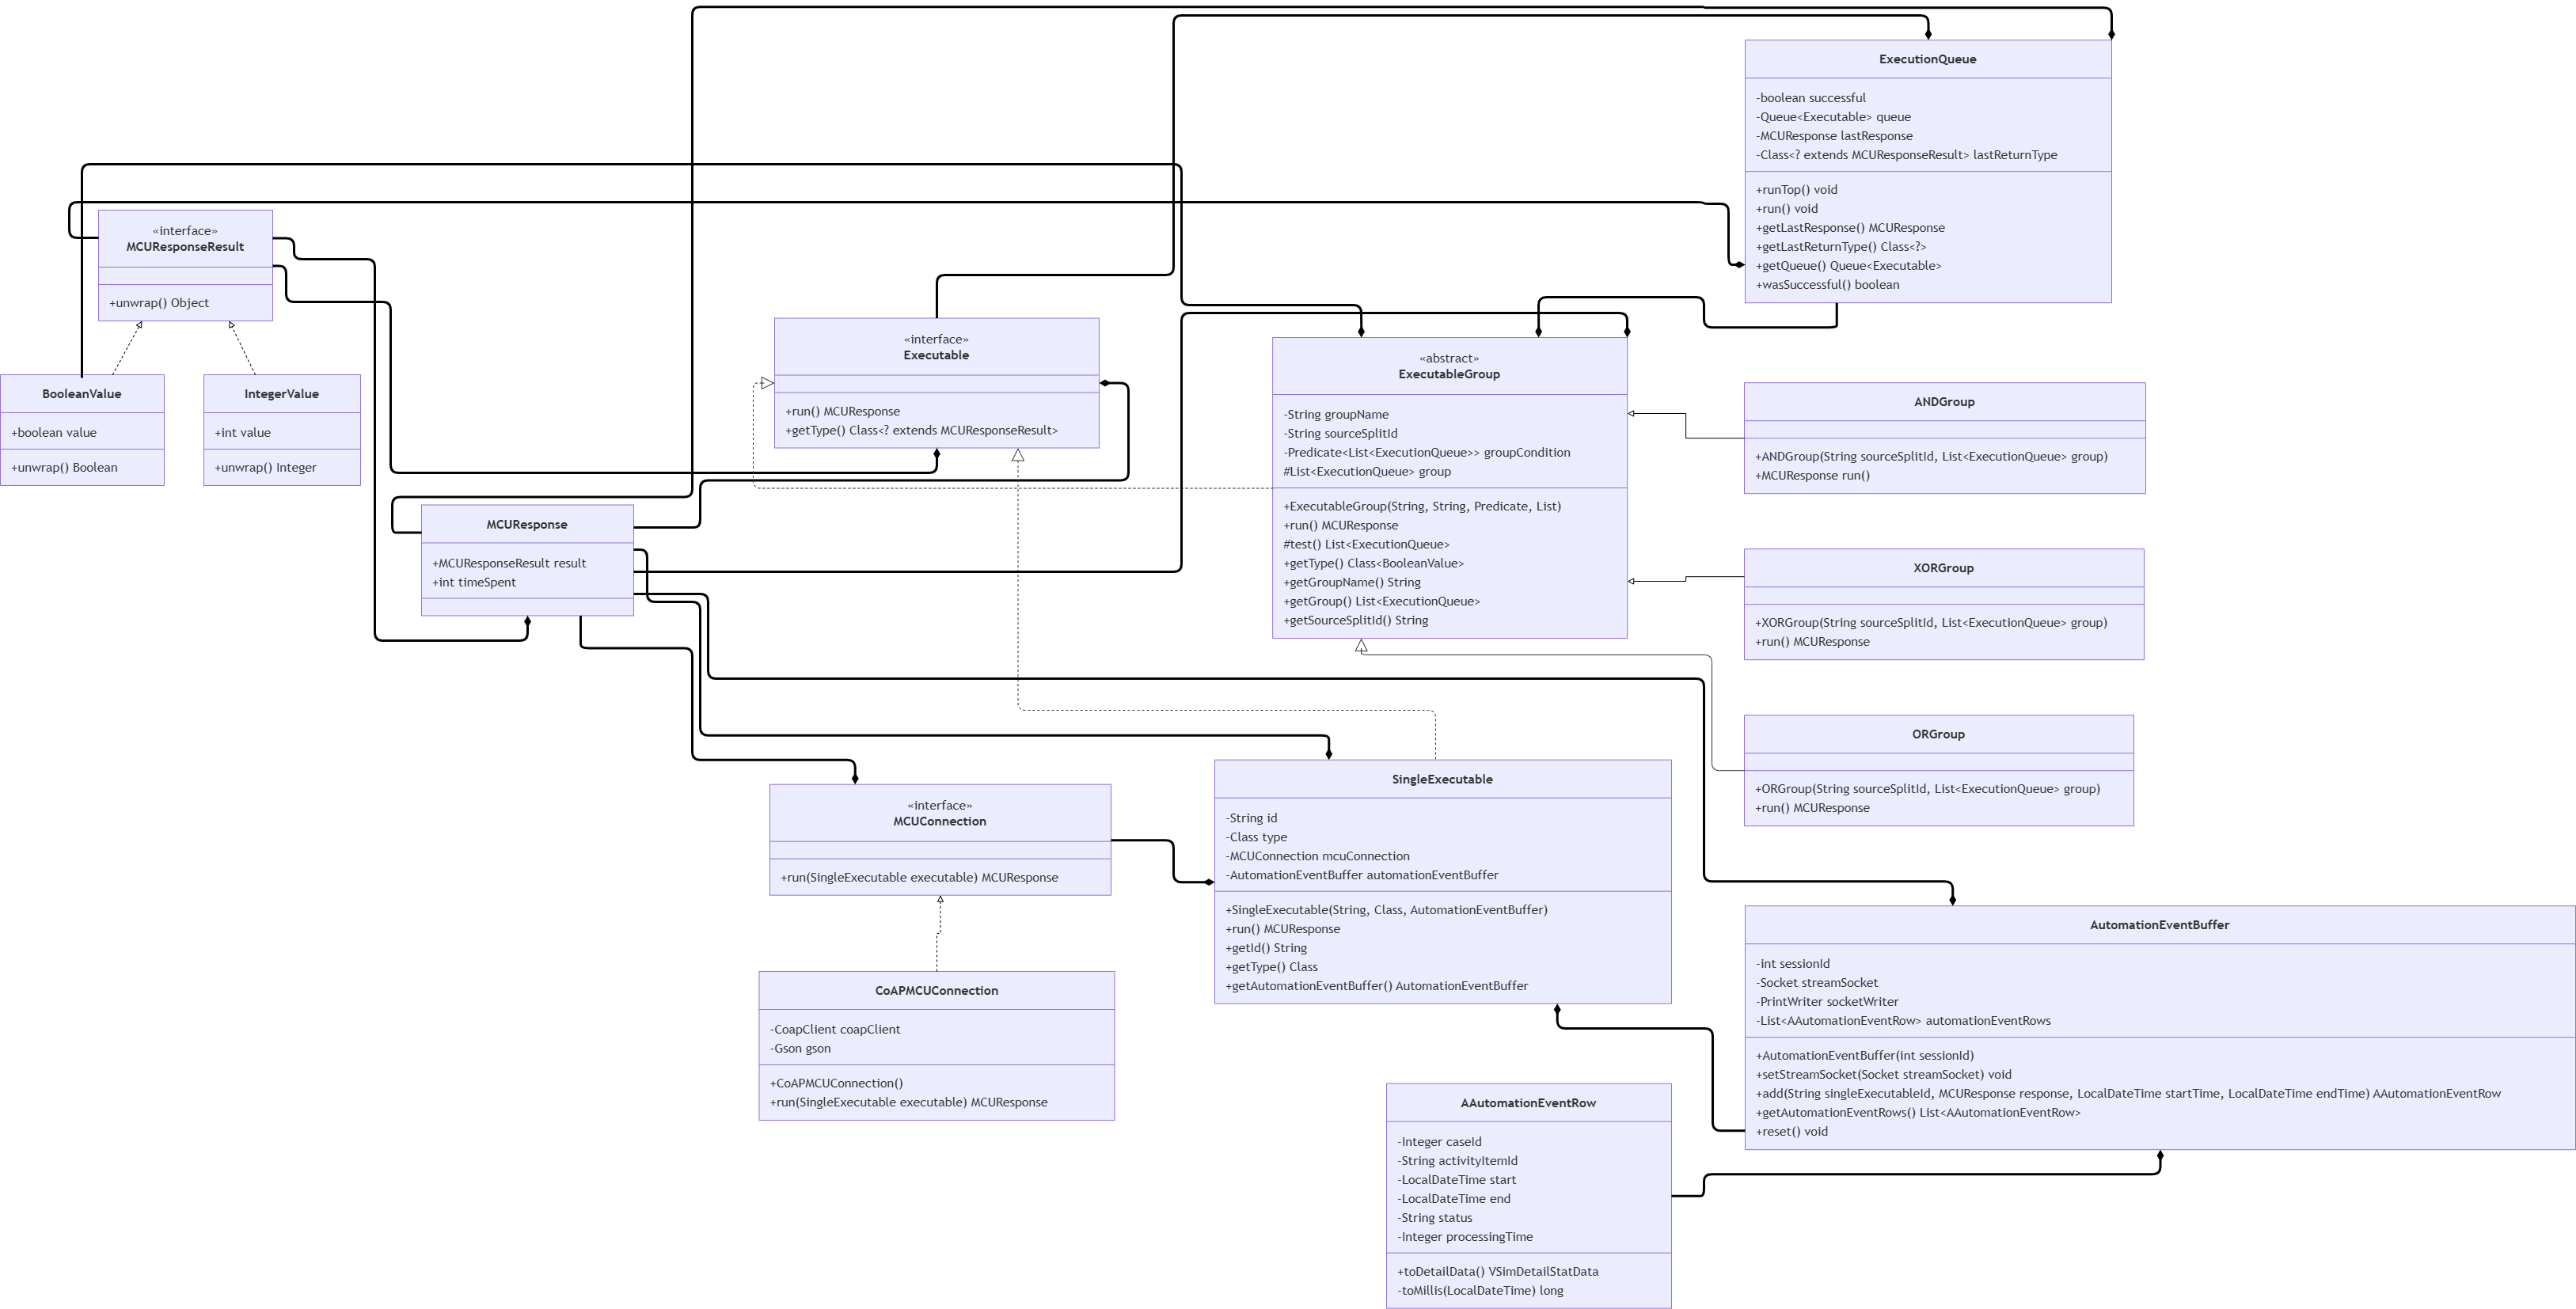
\includegraphics[width=0.8\textwidth]{Graphics/Ausführungsmodell-UML.png}
    \caption{UML Diagramm des Prozessmodellkonstruktionsklassen}
    \label{fig:process-builder-uml}
\end{figure}

Die einzelnen \texttt{*Extractor} Klassen erfüllen die Funktion, aus dem XML-Dokument die Elemente zu extrahieren. Diese Elemente werden in \texttt{ProcessExtractor} gesammelt
und zu einem \texttt{Process} (siehe \ref{fig:prozess-uml}) konstruiert. Nach der Konstruktion des \texttt{Process} Objekts wird die Vorverarbeitung durchgeführt, um $\tau$ zu
realisieren mittels \texttt{OperatorPreprocessor}.

\subsection{EPK-Compiler}
\label{epk-compiler}
Der Compiler wird in Java mit folgenden Klassen realisiert:

\begin{figure}[H]
    \centering
    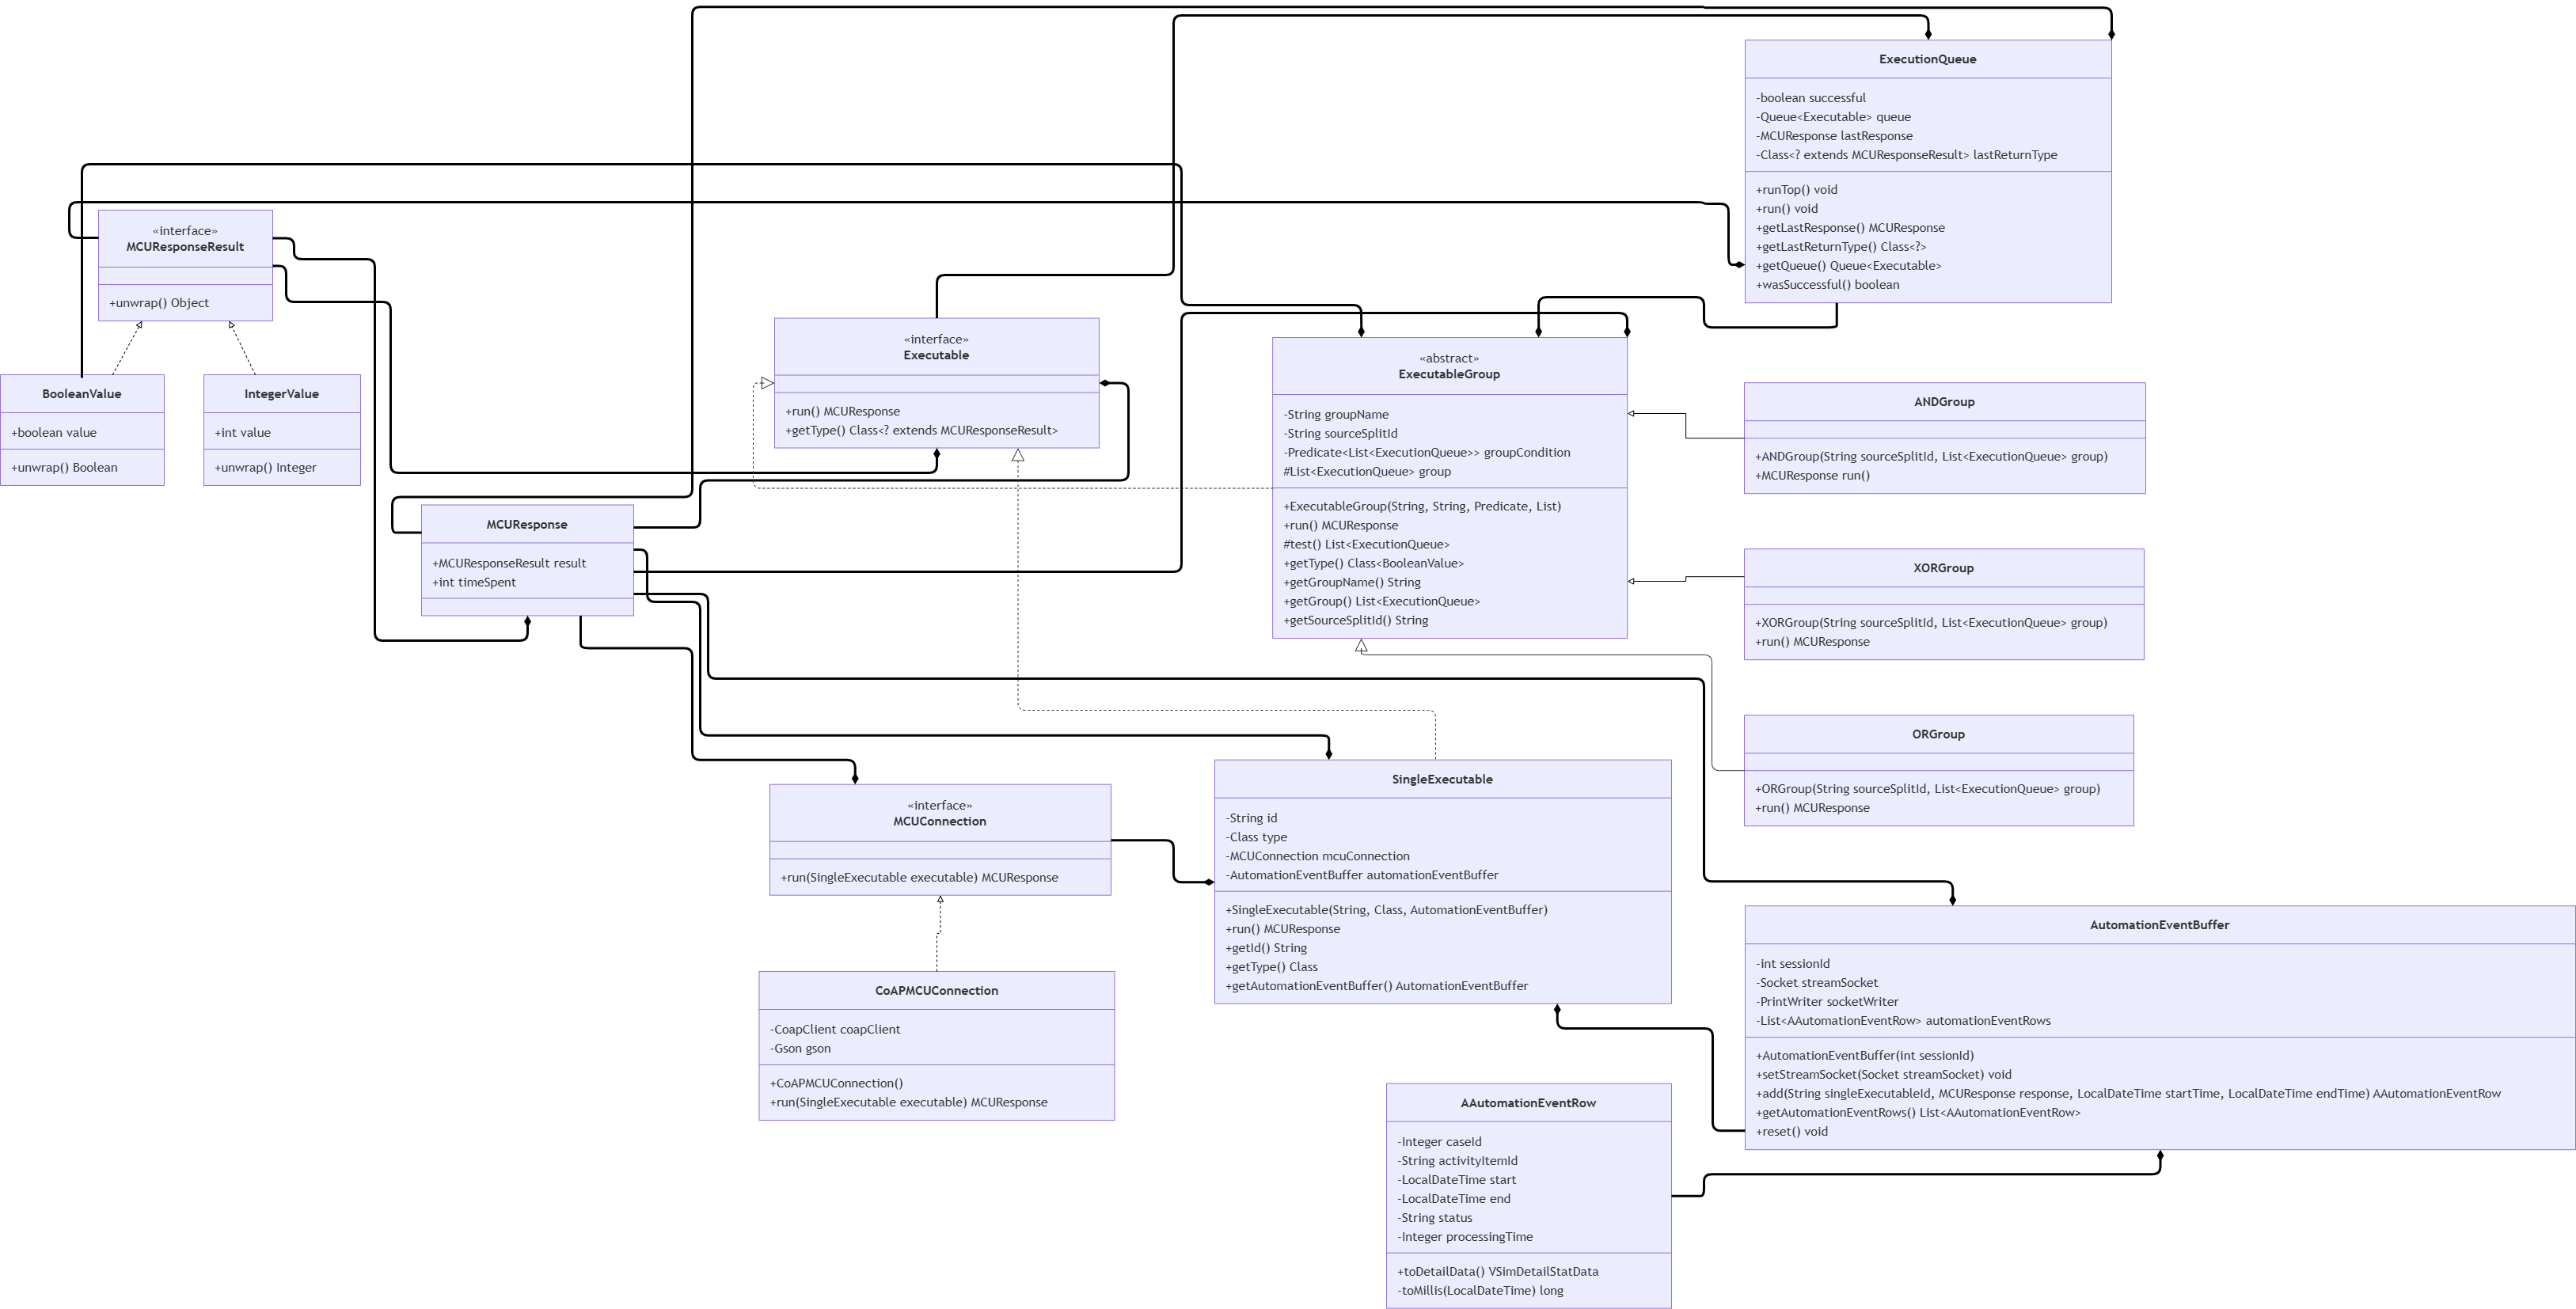
\includegraphics[width=0.8\textwidth]{Graphics/Ausführungsmodell-UML.png}
    \caption{UML Diagramm des EPK-Compilers}
    \label{fig:epk-compiler-uml}
\end{figure}

Der eigentliche EPK-Compiler ist \texttt{ExecutionQueueBuilder}. Dieser Funktioniert so, dass der aktuelle Kompilierzustand sich in \texttt{ExecutionQueueBuilderContext}
befindet. Dieser besteht aus einem Flag \texttt{started}, um zu wissen ob das Startereignis schon verarbeitet wurde, der zu füllenden ExecutionQueue und einem \texttt{Process}
Objekt. Zur Buchführung von Verknüpfungsoperatoren enthält der \texttt{ExecutionQueueBuilderContext} einen Stapel \texttt{groupDeque}, um die aktuell geöffnete Verknüpfung sich zu merken
und die Hash-Map \texttt{groupIndexMap}, um zu wissen welcher Pfad im aktuellen Verknüpfungsoperator verarbeitet wird. Dazu kommen noch eine \texttt{AutomationEventBuffer} Referenz, welche einem
\texttt{SingleExecutable} durchgegeben wird, um dessen Ausführung zu dokumentieren und eine verkettete Liste \texttt{SingleExecutables}, welche zur Codegenerierung verwendet wird.

Die Kompilierung findet wie folgt statt: Es wird durch den Prozessgraphen $G_P$ mittels Tiefensuche traversiert (durch \texttt{Utils.traverse}) und abhängig vom Knoten wird der passende \texttt{Handler} aus der 
\texttt{HandlerFactory} angefragt, um den Knoten zu verarbeiten. Sowohl \texttt{TaskHandler} als auch die einzelnen  \texttt{EventHandler} verarbeiten den Knoten zu einem \texttt{SingleExecutable} Objekt, welches
in der \texttt{ExeuctionQueue} des \texttt{ExecutionQueueBuilderContext} hinterlegt wird. \texttt{SplitOperatorHandler} und \texttt{JoinOperatorHandler} verarbeiten die Verknüpfungsoperatoren und verarbeiten die darin 
gekapselte Struktur zu einer \texttt{ExecutableGroup}.

\subsection{Ausführung des Ausführungsmodells}

Die Ausführung der \texttt{ExecutionQueue} wird mit einer \texttt{while} Schleife realisiert mit der Bedigung, dass die FIFO-Warteschlange nicht leer ist. 
Inital wird die erste \texttt{Executable} der \texttt{ExecutionQueue} entnommen und der Status der letzten Ausführung wird als erfolgreich markiert,
um die Ausführung zu starten. Der Rückgabetyp des \texttt{Executable} wird sich gemerkt, das \texttt{Executable} Objekt wird ausgeführt und der initiale 
Ausgabewert wird mit dem des durchgeführten \texttt{Executables} überschrieben. Der Ausführungsstatus wird durch Evaluation des Rückgabewertes (beim Rückgabetyp \text{int},
ob eine 0 zurückgegeben wurde; beim Rückgabetyp \texttt{bool}, ob \texttt{true} zurückgegeben wurde). Ist die \texttt{ExecutionQueue} noch gefüllt und der Rückgabewert indiziert
eine erfolgreiche Ausführung so wird die Schleife nochmal durchlaufen. Bei leerer \texttt{ExecutionQueue} oder einer vorherigen fehlerhaften Ausführung wird die Schleife und somit auch
die Ausführung der gesamten \texttt{ExecutionQueue} gestoppt.

\begin{figure}[H]
    \centering
    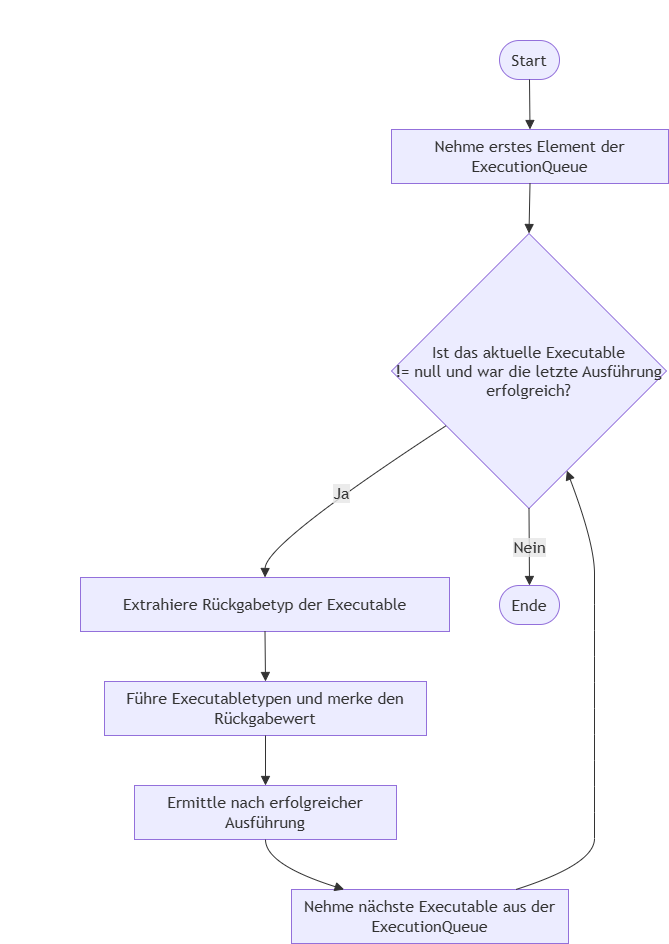
\includegraphics[width=0.8\textwidth]{Graphics/Ausführung-der-ExecutionQueue.png}
    \caption{Flussdiagram zur Ausführung der ExecutionQueue}
    \label{fig:flowchar-execution-queue}
\end{figure}


\subsection{IOT-Schnittstelle}
\label{iot-interface-impl}

Die IoT-Schnittstelle sendet die Befehle einer \texttt{SingleExecutable} zum IoT-System. Das IoT-System besteht dabei aus 
Microkontrollern. In dieser Arbeit Microkontroller der Reihe ESP32. Die Schnittstelle wird mit dem CoAP Protkoll realisiert.
Dabei wird die Realisierung eines Prozesses durch einen CoAP PUT-Endpoint realisiert. Anhand der Schnittstellendefinition 
aus \ref{coap-interface} entspricht der Pfadname eines Endpunktes den ersten 16 Zeichen eines SHA256-Hexstrings. 

Alle CoAP-Endpunkte, welche die Funktionalität des SingleExecutables zur Verfügung stellen werden beim Start des Servers aus
einem Resource-Directory abgefragt, welches die CoAP-URL's enthält. Das Ergebnis wird in einer Hash-Map hinterlegt, wo der gekürzte
SHA256-Hexstring der Schlüssel die CoAP-URL der Wert ist. Bei der Ausführung eines \texttt{SingleExecutable} wird durch die ID des \texttt{SingleExecutable}
genommen, der gekürzte Hexstring erzeugt, der CoAP-Pfad wird entnommen und die CoAP-Anfrage wird an direkt an den ESP32 verschickt.

\begin{figure}[H]
    \centering
    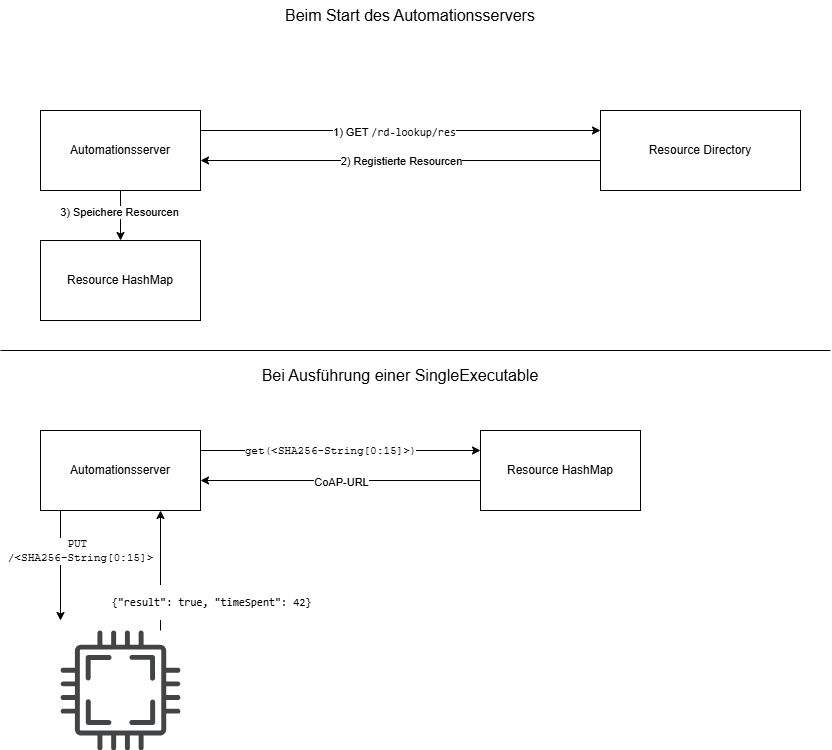
\includegraphics[width=0.8\textwidth]{Graphics/CoAP-SingleExecutable-Ausführung.png}
    \caption{Ausführung einer \texttt{SingleExecutable}}
    \label{fig:coap-single-executable-execution}
\end{figure}

\subsubsection{Pfadgenerierung durch SHA256}

Der SHA256-Hexstring aus \ref{iot-interface-impl} wird für jeden Knoten $(i, t) \in X_S$ erzeugt. Dafür 
wird $sha256(i)$ berechnet. Diese Prüfsumme wird in Java als Hexstring hinterlegt. Aus diesem Hexstring wird 
ein Substring aus den ersten 16-Zeichen entnommen. Dieser Substring ist die URI des Endpoints. Es wird so 
vorgegangen, da die ID in ARIS Zeichen enthält, welche für URIs nicht kompatibel sind. Zur Generierung des 
SHA256-Hexstrings wird Apache Commons verwendet, da Hashing mit mit Java-Boardmitteln Boilerplate-Code einführt, 
was die Lesbarkeit und Wartbarkeit des Codes negativ beeinflusst. 

\begin{figure}[H]
    \centering
    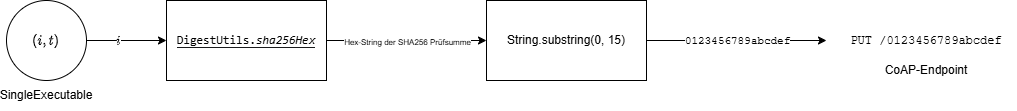
\includegraphics[width=0.8\textwidth]{Graphics/CoAP-Pfadgenerierung.png}
    \caption{CoAP-Pfadgenerierung}
    \label{fig:coap-path-generation}
\end{figure}

\subsubsection{Aufsetzen des Resource Directory Servers}

Bei dem Resource-Directory handelt es sich um \texttt{cf-rd}. Einer Resource-Directory Implementierung vom Eclipse Californium 
Projekt. Dieses wurde in ein Docker-Image überführt, sodass die Einrichtung effizient durchgeführt werden kann und auch 
Konfigurationsänderungen schneller umgesetzt werden können. Dieses Docker-Image wurde auf einer AWS-EC2 Instanz ausgeführt.

\section{Firmwarecodegenerierung}

Bei der Firmwarecodegenerierung werden alle SingleExecutable Instanzen durch JSON serialisiert und werden an ein Python-Skript übergeben, 
welches ein ESP-IDF Projekt anlegt und anhand der serialisierten SingleExecutables die einzelnen CoAP-Handler Klassen erzeugt.

\subsection{Integration in ESP-IDF}

Für den Firmwarecode wurde ESP-IDF als Basis genommen. Aspekte wie der Aufbau einer WLAN-Verbindung, die Initialisierung eines CoAP-Servers 
sowie Einrichtungscode eines CoAP-Endpoint Handlers sind schon eingebaut. Nach der Codegenerierung muss nur noch die Ausführungslogik implementiert
werden.

\begin{figure}[H]
    \centering
    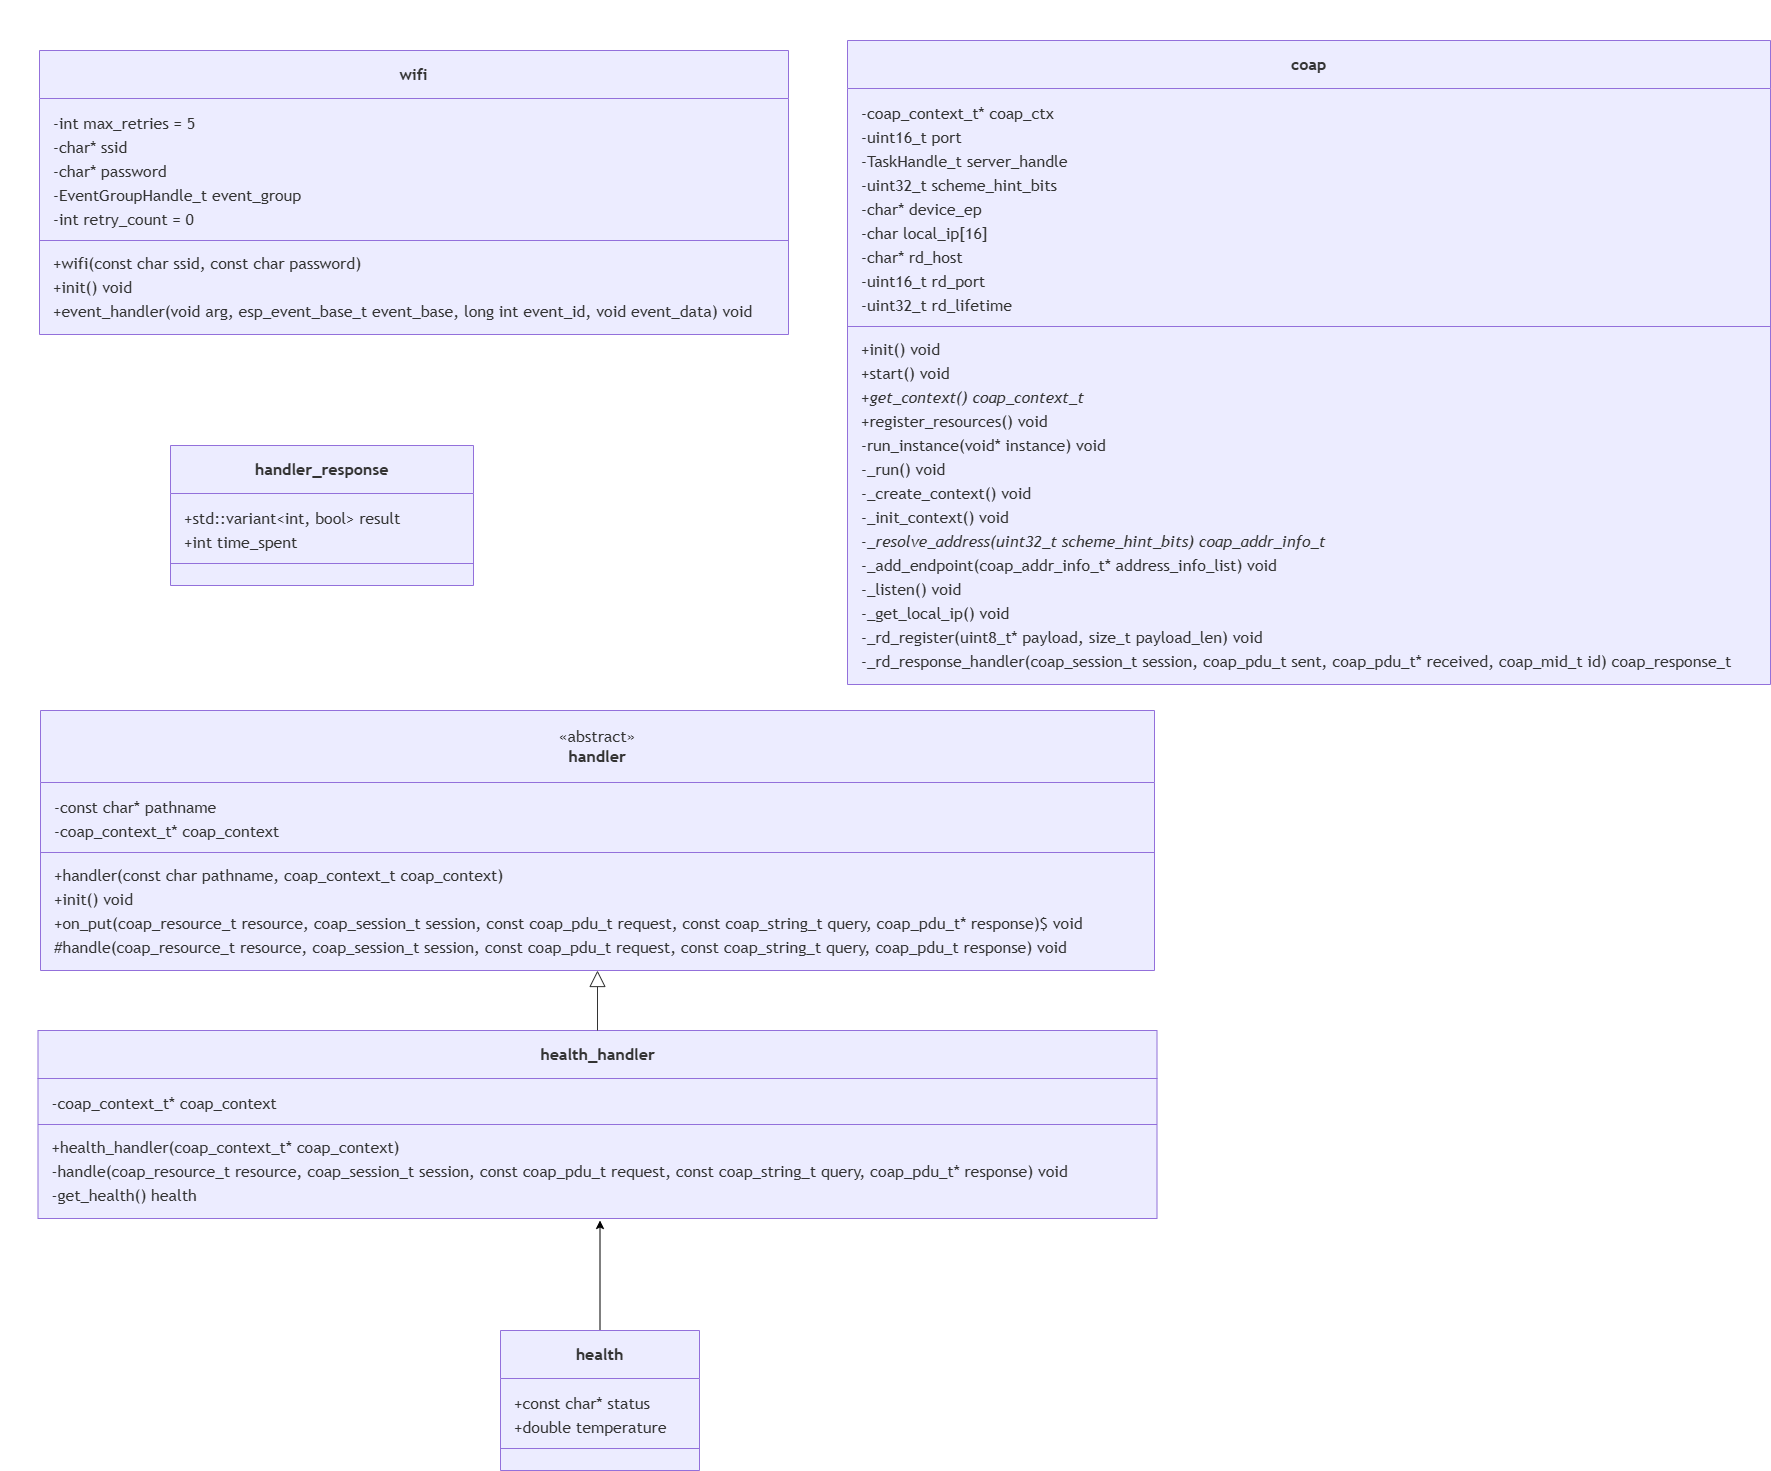
\includegraphics[width=0.8\textwidth]{Graphics/Firmware-UML.png}
    \caption{Klassen innerhalb eines generierten ESP-IDF Projekts}
    \label{fig:idf-project-classes}
\end{figure}

\subsection{Übersetzung des Ausführungsmodells in C++}

Aus \ref{epk-compiler} ist zu entnehmen, dass ein \texttt{ExecutionQueueBuilderContext} eine verkettete Liste an \texttt{SingleExecutable}
Instanzen enthält. Diese Liste wird mit JSON serialisiert und als JSON-Datei abgespeichert. Danach wird ein Python-Skript ausgeführt, welches 
dieses JSON-Dokument einliest und auf dieser Basis CoAP-Handler Klassen erstellt.

\begin{figure}[H]
    \centering
    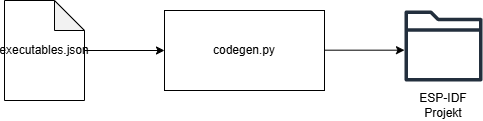
\includegraphics[width=0.8\textwidth]{Graphics/Codegen-Diagram.png}
    \caption{Work}
    \label{fig:idf-project-classes}
\end{figure}

\section{Ausgabe von Ausführungsstatistiken}
\section{Integration in ARIS}
\subsection{Ersetzen der Simulationsschnittstelle}
\subsection{Anpassung an der Nutzeroberfläche}
\subsection{Bereitstellung von Ausführungsstatistiken für ARIS Process Mining}
\subsection{Animation der Automatisierung}
